\subsection{Radiation Cloud Modelling}
The radiation cloud is assumed to be monitored using a number of sensors on the ground (within the disaster space) that collect readings every minute of the game. The radiation cloud diffusion process is modelled by a nonlinear Markov field stochastic differential equation, which assumes the cloud intensity is Gaussian distributed in log-space.  The cloud is driven by wind forces which vary both spatially and temporally.  Wind forces induce an anisotropic diffusion coefficient into the cloud diffusion process.  The wind velocity is modelled by two a priori independent Gaussian processes (GP), one GP for each Cartesian coordinate axis.  The GP captures both the spatial distribution of the wind velocity and also the dynamic process resulting from shifting wind patterns such as short term gusts and longer term variations.  In our simulation, each spatial wind velocity component is modelled by a squared-exponential GP covariance function, $K$, with fixed input and output scales over time (although any covariance function, stationary or not, can be substituted).

Both the radiation cloud and wind model priors are combined into a single joint model called a {\it latent force model} (LFM)~\cite{alvarez09} and predictions of the radiation cloud intensity are inferred using the extended Kalman filter (EKF).  The EKF provides both the mean and variance of the log-radiation cloud intensity and wind conditions.  Uncertainty arises due to unknown initial conditions of the cloud and wind conditions and it is also induced by the stochastic nature of their processes.  The EKF state $S(t)=(\underline{R}(t) \underline{V}_x(t) \underline{V}_y(t))^T$ represents both Cartesian components of the wind velocity, $V_x(t)$ and $V_y(t)$, and the log-radiation cloud density, $R(t)$, on a regular $N\times M$ grid defined across the environment with grid coordinates $G$.  The temporal component of the wind GP model is assumed Markovian and thus, the wind dynamics are incorporated within the EKF as per the KFGP~\cite{reece10}.  For example, the $N\times M$ x-component of the wind velocity at time-step $t+1$ is $V_x(t+1)=F V_x(t)+\nu_t$, where the process model $F=\rho I$ (where $I$ is the identity matrix) and Gaussian process noise $\nu_t\sim \Bbb{N}(0,(1-\rho^2) K(G,G))$ for correlation, $\rho$, of the wind field between time steps.  When $\rho=1$ the wind velocities are time invariant (although spatially variant).  Values of $\rho<1$ model wind conditions that change over time.
(\textbf{Steve: in the platform we take the `real' values from the diffusion process i believe. Does the above capture this? We will say that we will add the features you mention below to a future version of the platform where we aim to do both situational awareness and rescue. Add a sentence above to conclude where we took the values from and the process takes into account the  location of radiation source. Also, your notation clashes with the notations in the scenario and Feng's algorithm - please try to align.}
%The cloud intensity and wind velocity are measured by {\it monitor agents} equipped with geiger-counters and anemometers.  These agents are directed to take measurements with greatest information gain in the radiation cloud intensity.  The measurements are folded into the EKF and this refines estimates of the radiation cloud across the grid.  Figure~\ref{radiation_screen_shots} shows example cloud simulations for slow varying (i.e. $\rho=0.99$) and gusty (i.e. $\rho=0.90$) wind conditions.  Figure~\ref{radiation_screen_shots}(a) shows slow varying wind conditions in which case the radiation cloud can be interpolated accurately using sparse sensor measurements and the LFM model.  Alternatively, during gusty conditions the radiation cloud model is more uncertain far from the locations where recent measurements have been taken, as shown in Figure~\ref{radiation_screen_shots}(b).
%
%\begin{figure}[ht] \begin{center}
%    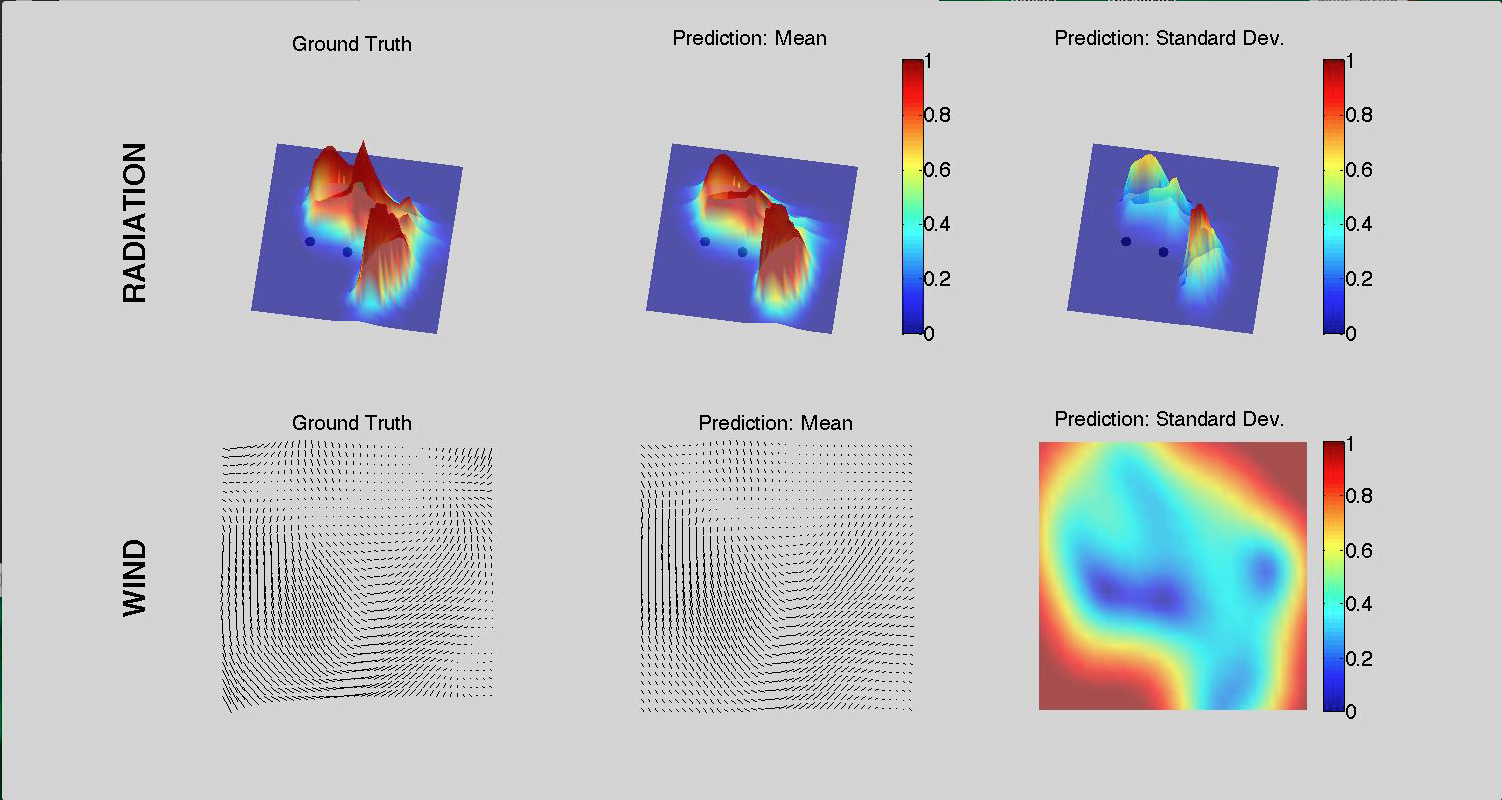
\includegraphics[width=0.45\textwidth]{figures/radiation_ss_calm.png}\\
%    (a) Slowly varying wind conditions\\ \ \\
%    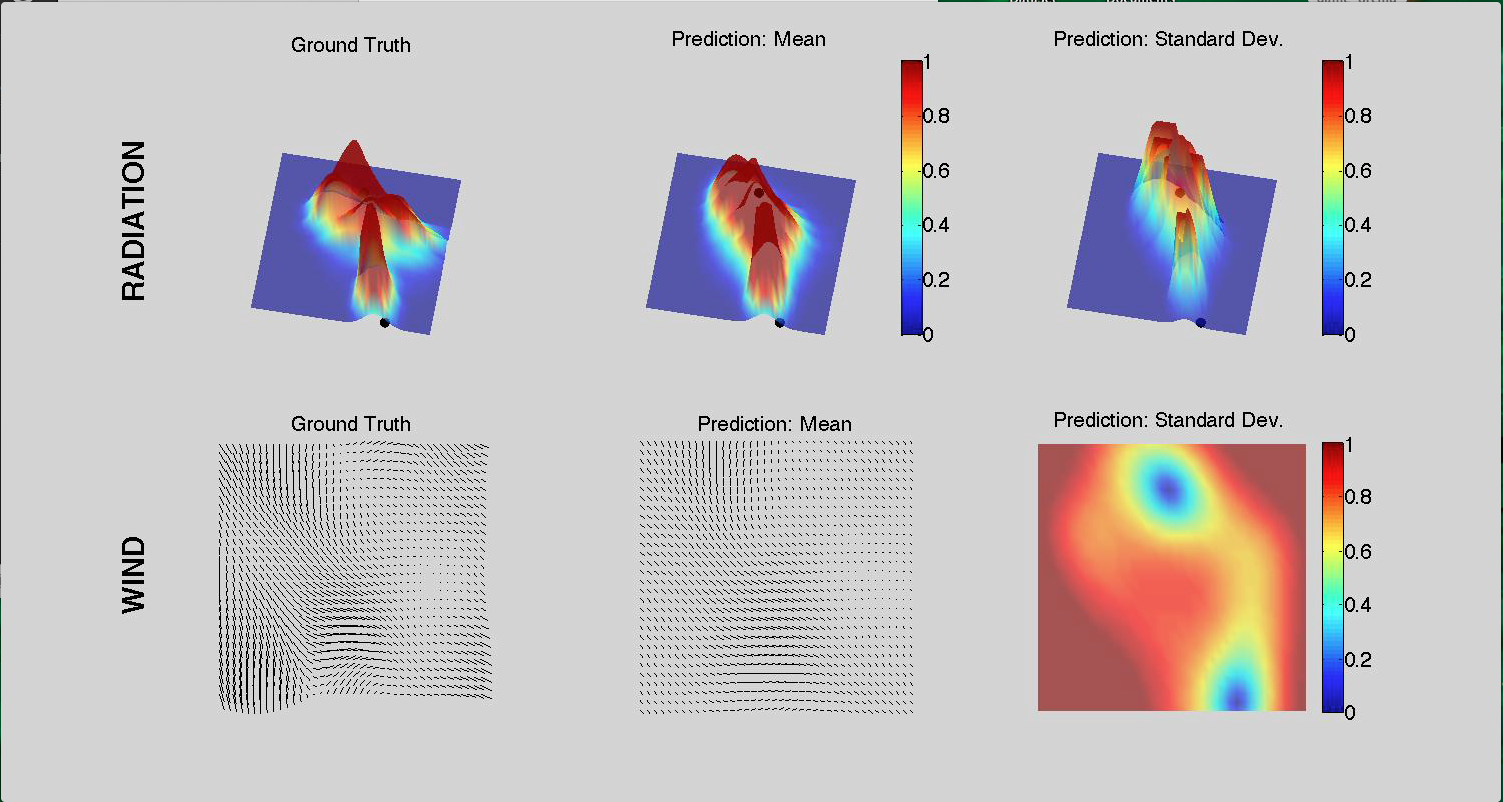
\includegraphics[width=0.45\textwidth]{figures/radiation_ss_gust.png}\\
%    (b) Gusty wind conditions 
%\caption{\label{radiation_screen_shots} Radiation and wind simulation ground truth and EKF estimates obtained using measurements from monitor agents (black dots).  Left most panes are ground truth radiation and wind conditions, the middle panes are corresponding estimates and right most panes are state uncertainties:  (a) Invariant and (b) gusty wind conditions.}
%\end{center}
%\end{figure}
